\documentclass[a4paper,11pt]{article}

\input ../include/preamble.tex

\usepackage{tikz}
\usetikzlibrary{automata,arrows,topaths,calc,positioning}

\usepackage{caption}
\usepackage{subcaption}


\begin{document}

\title{
    \textbf{Train shunting}\\
    \large{Programming II - Elixir Version}
}
\author{Christian Schulte \\ \\ {\em adapted to Elixir by Johan Montelius}}
\date{Spring Term 2023}
\maketitle


\thispagestyle{fancy}

\section*{Introduction}

You are in charge of shunting wagons of a train.  In
the following we assume that each wagon is self driving and that the
train has no explicit engine.

The description for your shunting task is given by two sequences of
wagons: the given train and the desired train. Your task is to
rearrange the given train with help of your shunting station such that
the desired train is obtained. You are not only supposed to rearrange
the train but also to compute a sequence of shunting moves (which are
called just ``moves'' from now on).


The shunting station is shown in Figure~\ref{fig:station}. It has a
``main'' track and two shunting tracks ``one'' and ``two''.  A
situation in the shunting station is called \emph{state}. A
\emph{move} describes how wagons move from one track to another.

\begin{figure}[h]
\begin{center}
  \begin{tikzpicture}
    \node(main) [rectangle, draw , minimum height=1cm, minimum width=3cm]{main};
    \node(one) [rectangle, draw, minimum height=1cm, minimum width=3cm, above right = 0.5cm and 4cm of main ]{one};
    \node(two) [rectangle, draw, minimum height=1cm, minimum width=3cm, below right = 0.5cm and 4cm of main]{two};
    \draw[<->] (main) to[out=0,in=180](one);
    \draw[<->] (main) to[out=0,in=180](two);    
  \end{tikzpicture}
\end{center}  
\caption{Train shunting station}
\label{fig:station}
\end{figure}

\paragraph{Goal}

Our ultimate goal in this lab is to find a short sequence
of moves that turn a train on the track ``main'' into another
configuration of the train on ``main''.


Before we attempt this goal we will fix the modeling of our
problem and develop some list processing support.

\paragraph{Lab purpose}

This lab exercises several important issues. How are problems modeled
by data structures such as lists and tuples. How are lists
processed. This ranges from simple to more complicated patterns of
recursion over lists. This lab is of course also geared at getting you
started with Erlang and functional programming in general.

And last, but not least, we hope that you have \emph{some fun} solving
this little puzzle.

\section*{Modeling}

\paragraph{Trains, wagons, and states}

Wagons are modeled as atoms and trains on tracks as lists of atoms. A
train has no duplicate wagons (that is, \verb+[:a,:b]+ is a train,
whereas \verb+[:a,:a]+ is not).

A complete description of the state of a shunting station
consists of three lists: a list describing the train on track
``main'', and two lists describing tracks ``one'' and ``two''.

\begin{figure}[h]
\begin{center}
  \begin{tikzpicture}
    \node(main) [rectangle, draw , minimum height=1cm, minimum width=3cm]{{\tt [:a, :b]}};
    \node(one) [rectangle, draw, minimum height=1cm, minimum width=3cm, above right = 0.5cm and 4cm of main ]{{\tt [:c, :d] }};
    \node(two) [rectangle, draw, minimum height=1cm, minimum width=3cm, below right = 0.5cm and 4cm of main]{{\tt [:e, :f]}};
    \draw[<->] (main) to[out=0,in=180] (one);
    \draw[<->] (main) to[out=0,in=180](two);    
  \end{tikzpicture}
\end{center}
\caption{Example state displayed.}
\label{fig:ex-state}
\end{figure}

\paragraph{right-most, left-most}

One important question is of course which wagons are the {\em
 right-most} and {\em left-most}. We can of course choose how we
represent our tracks but will chose a way that follows how we write our tracks.

For track one and two the first element in the list will be the wagon
closes to the path to the main track. The first element in the list
that represents the main track is the left-most wagon on the track
i.e. furthest from track one and two.

The state \verb+{[:a,:b],[:c, :d],[:e, :f]}+
is visualized in Figure~\ref{fig:ex-state}.


\paragraph{Moves}

A move is a binary tuple. The first element of a move is either
\verb+:one+ or \verb+:two+. The second element of a move is an
integer. For example, \verb+{:one,2}+, \verb+{:two,2}+, and
\verb+{:one,-3}+ are all moves.

\paragraph{Applying a move to a state}

Moves describe how one state is transformed into another:
\begin{itemize}
\item If the move is \verb+{:one,n}+ and \verb+n+ is greater than
  zero, then the \verb+n+ right-most wagons are moved from track
  ``main'' to track ``one''.

  If there are more than \verb+n+ wagons on track ``:main'', the
  other wagons remain.

\item If the move is \verb+{:one,n}+ and \verb+n+ is less than zero,
  then the \verb+n+ left-most wagons are moved from track ``one''
  to track ``main''.

  If there are more than \verb+n+ wagons on track ``one'', the
  other wagons remain.
\item The move \verb+{:one,0}+ has no effect.
\end{itemize}

The same holds true for moves with first element \verb+:two+
concerning track ``two''.


\begin{figure}[h]
\begin{center}
\begin{tabular}{lr}
  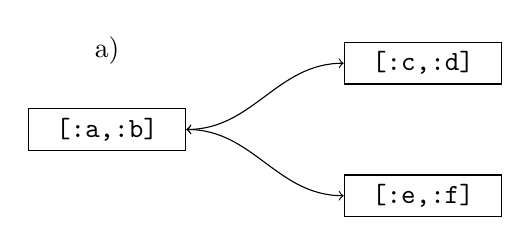
\begin{tikzpicture}
    \node(main) [rectangle, draw , minimum height=0.5cm, minimum width=2cm]{{\tt [:a,:b]}};
    \node(one) [rectangle, draw, minimum height=0.5cm, minimum width=2cm, above right = 0.3cm and 2cm of main ]{{\tt [:c,:d] }};
    \node(two) [rectangle, draw, minimum height=0.5cm, minimum width=2cm, below right = 0.3cm and 2cm of main]{{\tt [:e,:f]}};
    \draw[<->] (main) to[out=0,in=180](one);
    \draw[<->] (main) to[out=0,in=180](two);    
    \node(cap) [rectangle, above of=main] {a)};
  \end{tikzpicture} &
  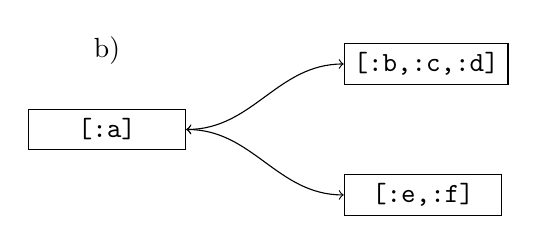
\begin{tikzpicture}
    \node(main) [rectangle, draw , minimum height=0.5cm, minimum width=2cm]{{\tt [:a]}};
    \node(one) [rectangle, draw, minimum height=0.5cm, minimum width=2cm, above right = 0.3cm and 2cm of main ]{{\tt [:b,:c,:d] }};
    \node(two) [rectangle, draw, minimum height=0.5cm, minimum width=2cm, below right = 0.3cm and 2cm of main]{{\tt [:e,:f]}};
    \draw[<->] (main) to[out=0,in=180](one);
    \draw[<->] (main) to[out=0,in=180](two);    
    \node(cap) [rectangle, above of=main] {b)};
  \end{tikzpicture}
  \\[1cm]
  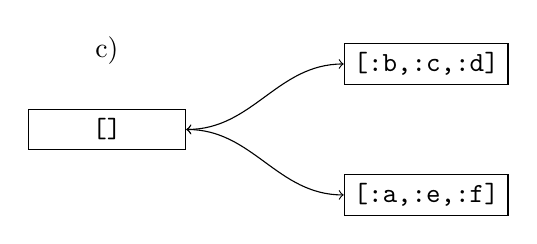
\begin{tikzpicture}
    \node(main) [rectangle, draw , minimum height=0.5cm, minimum width=2cm]{{\tt []}};
    \node(one) [rectangle, draw, minimum height=0.5cm, minimum width=2cm, above right = 0.3cm and 2cm of main ]{{\tt [:b,:c,:d] }};
    \node(two) [rectangle, draw, minimum height=0.5cm, minimum width=2cm, below right = 0.3cm and 2cm of main]{{\tt [:a,:e,:f]}};
    \draw[<->] (main) to[out=0,in=180] (one);
    \draw[<->] (main) to[out=0,in=180](two);    
    \node(cap) [rectangle, above of=main] {c)};
  \end{tikzpicture} &
  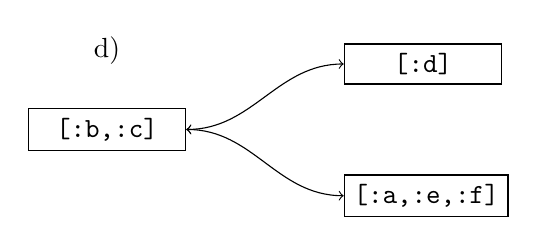
\begin{tikzpicture}
    \node(main) [rectangle, draw , minimum height=0.5cm, minimum width=2cm]{{\tt [:b,:c]}};
    \node(one) [rectangle, draw, minimum height=0.5cm, minimum width=2cm, above right = 0.3cm and 2cm of main ]{{\tt [:d] }};
    \node(two) [rectangle, draw, minimum height=0.5cm, minimum width=2cm, below right = 0.3cm and 2cm of main]{{\tt [:a,:e,:f]}};
    \draw[<->] (main) to[out=0,in=180](one);
    \draw[<->] (main) to[out=0,in=180](two);    
    \node(cap) [rectangle, above of=main] {d)};
  \end{tikzpicture}
\end{tabular}
\end{center}
\caption{Moves applied to states.}
\label{fig:ex-moves}
\end{figure}

\paragraph{Example}

Figure~\ref{fig:ex-moves} shows examples of moves applied to
states, where (a)~is the initial state, (b)~after application of
\verb+{:one,1}+, (c)~after application of \verb+{:two,1}+, and finally
(d)~after application of \verb+{:one,-2}+ (note the order).

\section*{Some train processing}

Before we actually start, we will develop some train-processing
routines that you will need later. When implementing these functions
you should implement them from scratch i.e. not use library modules
such as Lists, Enum etc. Why - because you will practice writing
recursive functions.


\begin{enumerate}

\item \verb+take(train,n)+ returns the train containing the first \verb+n+
  wagons of \verb+train+.

\item \verb+drop(train,n)+ returns the train \verb+train+ without its first
  \verb+n+ wagon.

\item \verb+append(train2,train2)+ returns the train that is the
  combinations of the two trains.

  For example,\verb+append([:a,:b],[:c])+ returns \verb+[:a, :b, :c]+.
  
\item \verb+member(train,y)+ tests whether \verb+y+ is a wagon of \verb+train+.

\item \verb+position(train,y)+ returns the first position (1 indexed) of \verb+y+ in
  the train \verb+train+. You can assume that \verb+y+ is a wagon in
  \verb+train+.

  For example, \verb+position([:a,:b,:c],:b)+ returns \verb+2+.

\item \verb+split(train, y)+ return a tuple with two trains, all the
  wagons before \verb+y+ and all wagons after \verb+y+
  (i.e. \verb+y+ is not part in either).

  For example: 
\begin{verbatim}
   split([:a,:b,:c],:a) = {[],[:b,:c]}

   split([:a,:b,:c],:b) = {[:a],[:c]}
\end{verbatim}

\item \verb+main(train, n)+ returns the tuple
  \verb+{k, remain, take}+ where \verb+remain+ and \verb+take+ are the
  wagons of \verb+train+ and \verb+k+ are the numbers of wagons
  remaining to have \verb+n+ wagons in the taken part.

  For example:
\begin{verbatim}
  main([:a, :b, :c, :d], 3) = {0, [:a], [:b, :c, .d]}

  main([:a, :b, :c, :d], 5) = {1, [], [:a, :b, :c, .d]}
\end{verbatim}  

\end{enumerate}

The last function requires some explanation; the wagons on the main
track are in reverse order i.e. the first wagon in the list is in the
leftmost position on the track. When you're asked to  move two
wagons to another track you should dive the train into two segments;
the segment that should remain and the two wagons (to the right i.e. in
the end of the list) that should be moved.

You could of course implement this by first counting the number of
wagons on the track and then decide how many to take and drop, but why
not do this in one recursive function? Implement the function
\verb+main/2+ as one recursive function without using the functions
that you have used before. In the report, describe how you have
implemented the function.

Please put all definitions together in one module {\tt Train} in a
file \verb+train.ex+


\section*{Applying moves}

The first task is writing a binary function \verb+single/2+ that
takes a move and an input state. It returns a
new state computed from the state with the move applied.

For example, \verb+single({:one,1},{[:a,:b],[],[]})+ returns
\verb+{[:a],[:b],[]}+.

\verb+single+ should be used later in this assignment whenever a
move is to be performed on a state.

Approach the task as follows:
\begin{itemize}
  
\item Your program should decide by pattern-matching which track
  is involved and what the different elements of a state are.
  
\item For a track, you have to decide whether wagons are moved
  \emph{on} or \emph{from} the track (that is, is \verb+n+  positive
  or negative).
  
\item Take into account that moves are allowed where no wagons
  are moved at all!

\item Use the \verb+main/2+ function when moving wagons from the main
  track.
\end{itemize}


You should also implement a function {\tt sequence/2}
that takes a list of moves and a state an returns a list of states
that that represents the transitions when the moves are performed.
For example,

\begin{verbatim}
 sequence([{:one, 1}, {:two, 1}, {:one, -1}, {:two, -1}], {[:a,:b], [], []})
\end{verbatim}

should return the lists:

\begin{verbatim}
[
  {[:a, :b], [], []},
  {[:a], [:b], []},
  {[], [:b], [:a]},
  {[:b], [], [:a]},
  {[:b, :a], [], []}
]
\end{verbatim}

You can use this function to verify that the sequences of moves that
you generate actually do solve the problem given.

Please store your function in a module called \verb+Moves+ in the file {\tt moves.ex}.


\section{The shunting problem}

So now for the actual problem, finding a sequence of moves that
changes the order of the wagons on the main track.

Develop a procedure \verb+find+ that takes two trains \verb+xs+
and \verb+ys+ as input and returns a list of moves, such that the
moves transform the state \verb+{xs,[],[]}+ into
\verb+{ys,[],[]}+.

In the following, we require that \verb+xs+ and \verb+ys+ contain the
same elements (wagons) and that each wagon is unique (in other
words, \verb+xs+ and \verb+ys+ are permutations of each other).

Approach the problem as follows. The problem is solved
recursively and each recursive step will move one wagon in the
position as required by \verb+ys+.

The base-case is simple. If there are no wagons, no moves are
needed.

Otherwise, we take the left-most wagon \verb+y+ from \verb+ys+ (the desired
train). Our goal is to find a list of moves that takes the wagon
\verb+y+ from its current position in \verb+xs+ to being the left-most
wagon in a train on the main track. This is done by the following
moves:

\begin{enumerate}
  
\item Split the train \verb+xs+ into the wagons \verb+hs+ and
  \verb+ts+, where \verb+hs+ are the wagons before \verb+y+
  in \verb+xs+, and \verb+ts+ are the wagons after \verb+y+ in \verb+xs+.

\item Move \verb\verb+y+ and the following wagons (that is \verb+ts+) to track
  ``one''.
  
\item Move the remaining wagons (that is, \verb+hs+) to track
  ``two''.
  
\item Move all wagons on ``one'' to ``main'' (this includes \verb+y+,
  which goes as needed to the left-most position on ``main'').
  
\item Move all wagons on ``two'' to ``main''.
\end{enumerate}

After having moved one wagon in the right position, we only need to
consider the remaining wagons of \verb+ys+. We should of course update
the current state on the main track but the state is simply \verb+ts+
appended to \verb+hs+ (we moved \verb+ts+ to the main track before \verb+hs+).

Note that the function \verb+find/2+ does not need to "perform" the
moves using \verb+single/2+ or \verb+sequence/2+, we know what the
final state should look like. You can, or should, use \verb+sequence/2+
to verify that \verb+find/2+ actually takes us from the initial state
to the desired.

Please store your functions in the module \verb+Shunt+ (and file
\verb+shunt.ex+).

\paragraph{Example.}
Given the input train \verb+[:a,:b]+ and the output train \verb+[:b,:a]+, the
list of moves computed by \verb+find+ is:

\begin{verbatim}
   [{:one,1},{:two,1},{:one,-1},{:two,-1} 
    {:one,1},{:two,0},{:one,-1},{:two,0}]
\end{verbatim}

\section*{Finding less moves}

As you probably noticed, a generated sequence of moves contains a lot
of redundant moves. Develop a function \verb+few+ that behaves as
\verb+find+ but that takes for each recursive application into account
whether the next wagon is already in the right position. If so, no
moves are needed.

Proceed by modifying (only very few modifications are needed)
your program for \verb+find/2+.

Please store \verb+few/2+ also in the module \verb+Shunt+.

\paragraph{Example.}
Given the input train \verb+[:c,:a,:b]+ and the output train
\verb+[:c,:b,:a]+, the list of moves computed by \verb+few+ is:
\begin{verbatim}
   [{:one,1},{:two,1},{:one,-1},{:two,-1}]
\end{verbatim}


\section{Move compression}

The list of moves computed by \verb+few/2+ is still awkward and
can be easily optimized according to the following rules:
\begin{enumerate}
\item Replace \verb+{:one,n}+ directly followed by \verb+{:one,m}+ with
  \verb-{:one,n+m}-.
\item Replace \verb+{:two,n}+ directly followed by \verb+{:two,m}+ with
  \verb-{:two,n+m}-.
\item Remove \verb+{:one,0}+.
\item Remove \verb+{:two,0}+.
\end{enumerate}

These optimizations are \emph{correct} in the sense that the
shorter list of moves will compute the same final state.

This task is actually tricky: think for example of 
\begin{verbatim}
   [{:two,-1},{:one,1},{:one,-1},{:two,1}]
\end{verbatim}
Repeatedly applying the rules from above actually results in no
moves at all. By application of Rule~1 we obtain
\verb+[{:two,-1},{:one,0},{:two,1}]+;
by Rule~3 
\verb+[{:two,-1},{:two,1}]+;
by Rule~2
\verb+[{:two,0}]+;
and finally by Rule~4
\verb+[]+.

Develop a function \verb+compress/1+ that takes a list of moves and
returns a compressed list of moves. Compression must be complete,
that is, none of the above rules should be applicable to the
returned list of moves.

Approach this task as follows. Develop a procedure
\verb+rules/1+ that applies rules recursively. Then repeat
application of \verb+rules/1+ until the list of moves does not
change. Thus, \verb+compress+ is implemented as follows:
\begin{verbatim}
def compress(ms) do
    ns = rules(ms)
    if ns == ms do 
       ms
    else
       compress(ns)
    end
end
\end{verbatim}

Please store your program also in the module \verb+Shunt+.

\section{Finding really few moves}

\emph{This assignment is voluntary.} This means you don't have to
do it, however we strongly encourage you to do it. And actually
it is fun!

The problem with both \verb+find/2+ and \verb+few/2+ is that they
always push back the wagons from ``one'' and ``two'' to ``main'',
even though there might be some opportunity to actively use track
``two'' to push wagons from track ``one'' into position and vice
versa. In the following, we are going to take advantage of this.

Develop a procedure \verb+fewer+, that takes four arguments:
\verb+ms+ as the wagons on ``main'', \verb+os+ as the wagons on ``one'',
\verb+ts+ as the wagons on ``two'', and \verb+ys+ as the desired train.

\verb+fewer+ works recursively and as before, each recursive
invocation will bring the first wagon \verb+y+ of \verb+ys+ into the right
position. What is new, is that this wagon might be on either
track:
\begin{itemize}
\item If \verb+y+ is a member of \verb+ms+, bring it in the right
  position as done previously. Leave the other wagons on track
  ``one'' and ``two''.
\item If \verb+y+ is a member of \verb+os+ (it is on track ``one''), move
  the wagons in front first to ``main'' and then to ``two''. Then
  move \verb+y+ into position. Otherwise, leave the wagons on ``one''
  and ``two'' unchanged.

  This adds one more wagon in the right position on ``main''.
\item Do the same for ``two''.
\end{itemize}

Each recursive application of \verb+fewer+ has of course to
supply the wagons on all three tracks correctly!

Initially, \verb+fewer+ is applied such that the tracks ``one''
and ``two'' are the empty list. For example,
\begin{verbatim}
   fewer([:a,:b],[],[],[:b, :a])
\end{verbatim}
returns
\begin{verbatim}
   [{:one,1},{:two,1},{:one,-1},{:two,0},{:one,0},{:two,-1}]
\end{verbatim}

\section{Acknowledgments}

The idea and the initial problem formulation is taken from an
assignment at the 8'th Prolog Programming Competition organized by Bart
Demoen and Phuong-Lan Nguyen. 

\end{document}
